% ==================================================
% FIFO Data Structure
% Author: Lester James V. Miranda
% ==================================================

\documentclass[preview, convert={outfile=\jobname.png,density=300}]{standalone}

\usepackage{tikz}
\usepackage{color}
\usepackage{subfig}
\usepackage{ifthen}
\usepackage{graphicx}

\renewcommand\familydefault{\sfdefault}

\usetikzlibrary{
    matrix,
    shapes,
    fit,
    arrows,
    positioning,
    calc,
    backgrounds,
    shadows.blur,
    shapes.multipart,
    shapes.geometric,
}

\begin{document}
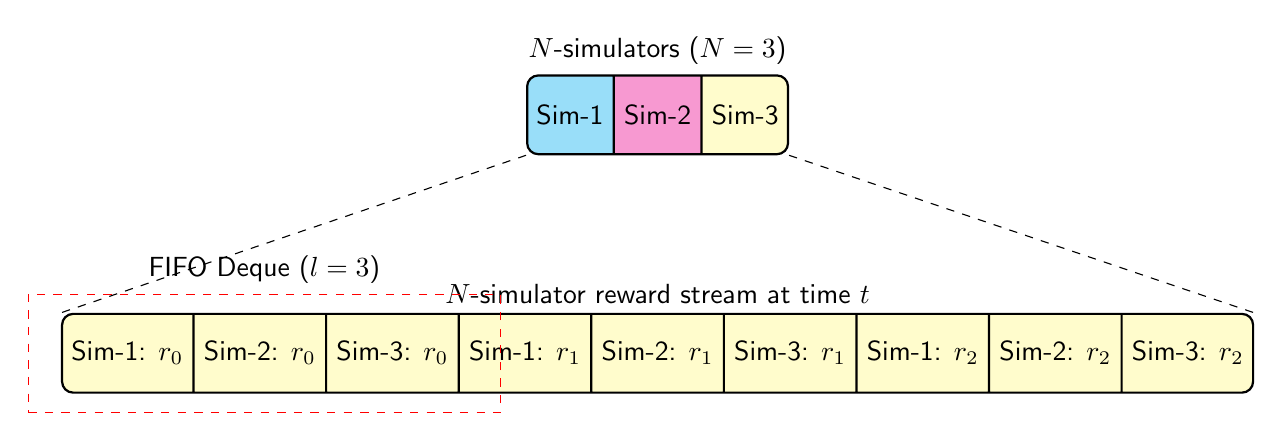
\begin{tikzpicture}[
    node distance= 2cm,
    deque/.style={draw, rectangle split, rectangle split horizontal, 
                   draw, text centered, rounded corners=4pt,
                   minimum width=12cm, minimum height=10mm, thick},
    fifo/.style={draw, rectangle, color=red, fill=none, dashed, anchor=west, minimum width=6cm, minimum height=1.5cm}
]

\node[deque, rectangle split parts=9, rectangle split part fill={yellow!20},
    label={[align=center] $N$-simulator reward stream at time $t$}]
    (rewardStream) at (0,0)
    {
        Sim-1: $r_0$
        \nodepart{second} Sim-2: $r_0$
        \nodepart{third} Sim-3: $r_0$
        \nodepart{four} Sim-1: $r_1$
        \nodepart{five} Sim-2: $r_1$
        \nodepart{six} Sim-3: $r_1$
        \nodepart{seven} Sim-1: $r_2$
        \nodepart{eight} Sim-2: $r_2$
        \nodepart{nine} Sim-3: $r_2$

    };

\node[deque, rectangle split parts=3, rectangle split part fill={cyan!40, magenta!40, yellow!20}, label={[align=center] $N$-simulators ($N=3$)}]
    [above=of rewardStream] (simulators)
    {
        Sim-1
        \nodepart{second} Sim-2
        \nodepart{third} Sim-3
    };

\node[fifo, label={FIFO Deque ($l=3$)}] at (-8,0) {};
\draw[-,dashed] (simulators.south west) -- (rewardStream.north west) {};
\draw[-,dashed] (simulators.south east) -- (rewardStream.north east) {};

\end{tikzpicture}
\end{document}


